\documentclass[border=8pt]{standalone}
\usepackage[T1]{fontenc}\usepackage[utf8]{inputenc}
\usepackage{helvet}\renewcommand{\familydefault}{\sfdefault}
\usepackage{tikz,xcolor}
\usetikzlibrary{arrows.meta,positioning,shapes.geometric,shapes.multipart,calc,fit,backgrounds,decorations.markings}
\definecolor{ink}{HTML}{1E1B16}\definecolor{paper}{HTML}{FBF8F2}\definecolor{clay}{HTML}{B5482A}\definecolor{soft}{HTML}{F1E9DA}\definecolor{pine}{HTML}{24402F}
\tikzset{
  every node/.style={font=\small,text=ink},
  >=Stealth, line/.style={draw=ink,line width=0.8pt},
  cls/.style={rectangle split,rectangle split parts=3,draw=ink,line width=0.8pt,fill=soft,align=left,inner xsep=6pt,inner ysep=4pt,
              rectangle split part align={center,left,left},minimum width=3.0cm},
  cls2/.style={rectangle split,rectangle split parts=2,draw=ink,line width=0.8pt,fill=soft,align=left,inner xsep=6pt,inner ysep=4pt,
              rectangle split part align={center,left},minimum width=3.0cm},
  box/.style={rectangle,draw=ink,line width=0.8pt,fill=soft,align=center,inner sep=5pt,minimum height=0.8cm},
  state/.style={rectangle,rounded corners=8pt,draw=ink,line width=0.8pt,fill=soft,align=center,inner sep=6pt,minimum width=2.2cm,minimum height=0.9cm},
  act/.style={rectangle,rounded corners=10pt,draw=ink,line width=0.8pt,fill=soft,align=center,inner sep=5pt,minimum width=2.4cm,minimum height=0.8cm},
  dec/.style={diamond,draw=ink,line width=0.8pt,fill=soft,inner sep=1pt,minimum width=0.9cm,minimum height=0.9cm},
  uc/.style={ellipse,draw=ink,line width=0.8pt,fill=soft,align=center,inner sep=3pt,minimum width=3.2cm,minimum height=1.0cm},
  note/.style={rectangle,draw=ink,line width=0.6pt,fill=yellow!12,align=left,inner sep=4pt,font=\footnotesize},
  lab/.style={font=\footnotesize,fill=paper,inner sep=1.5pt},
  err/.style={},
}
\newcommand{\actor}[3]{% x,y,label
  \draw[line width=0.8pt] (#1,#2+0.55) circle (0.17);
  \draw[line width=0.8pt] (#1,#2+0.38)--(#1,#2-0.15) (#1-0.3,#2+0.22)--(#1+0.3,#2+0.22) (#1,#2-0.15)--(#1-0.25,#2-0.6) (#1,#2-0.15)--(#1+0.25,#2-0.6);
  \node[font=\small] at (#1,#2-0.9) {#3};}
\begin{document}
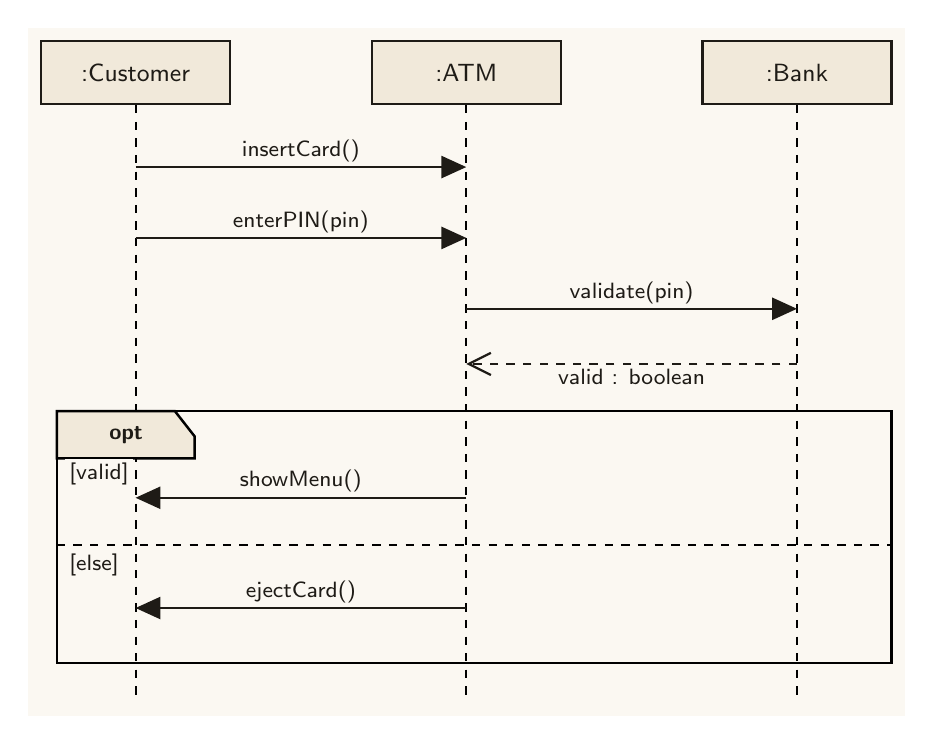
\begin{tikzpicture}[background rectangle/.style={fill=paper},show background rectangle]
\node[box,minimum width=2.4cm] (c) at (0,0) {:Customer};
\node[box,minimum width=2.4cm] (a) at (4.2,0) {:ATM};
\node[box,minimum width=2.4cm] (k) at (8.4,0) {:Bank};
\draw[dashed,line width=0.7pt] (c.south)--(c.south |- 0,-8.0);
\draw[dashed,line width=0.7pt] (a.south)--(a.south |- 0,-8.0);
\draw[dashed,line width=0.7pt] (k.south)--(k.south |- 0,-8.0);
\draw[line,-{Triangle[length=9pt,width=8pt]}] (0,-1.2)--(4.2,-1.2) node[midway,above,lab]{insertCard()};
\draw[line,-{Triangle[length=9pt,width=8pt]}] (0,-2.1)--(4.2,-2.1) node[midway,above,lab]{enterPIN(pin)};
\draw[line,-{Triangle[length=9pt,width=8pt]}] (4.2,-3.0)--(8.4,-3.0) node[midway,above,lab]{validate(pin)};
\draw[line,dashed,-{Straight Barb[length=8pt,width=8pt]}] (8.4,-3.7)--(4.2,-3.7) node[midway,below,lab]{valid : boolean};
\draw[line width=0.9pt] (-1.0,-4.3) rectangle (9.6,-7.5);
\draw[line width=0.9pt,fill=soft] (-1.0,-4.3)--(0.5,-4.3)--(0.75,-4.62)--(0.75,-4.9)--(-1.0,-4.9)--cycle;\node[font=\footnotesize\bfseries] at (-0.12,-4.6) {opt};
\node[lab,anchor=west] at (-0.9,-5.1) {[valid]};
\draw[line,-{Triangle[length=9pt,width=8pt]}] (4.2,-5.4)--(0,-5.4) node[midway,above,lab]{showMenu()};
\draw[dashed,line width=0.7pt] (-1.0,-6.0)--(9.6,-6.0);
\node[lab,anchor=west] at (-0.9,-6.25) {[else]};
\draw[line,-{Triangle[length=9pt,width=8pt]}] (4.2,-6.8)--(0,-6.8) node[midway,above,lab]{ejectCard()};
\end{tikzpicture}
\end{document}
